\section{Additional Analysis on \swebenchlite}

\subsection{Problem Classification}
\label{sec:benchmark_analysis}


\begin{figure*}[h]
\centering
    \begin{subfigure}[b]{0.33\textwidth}
        \centering
        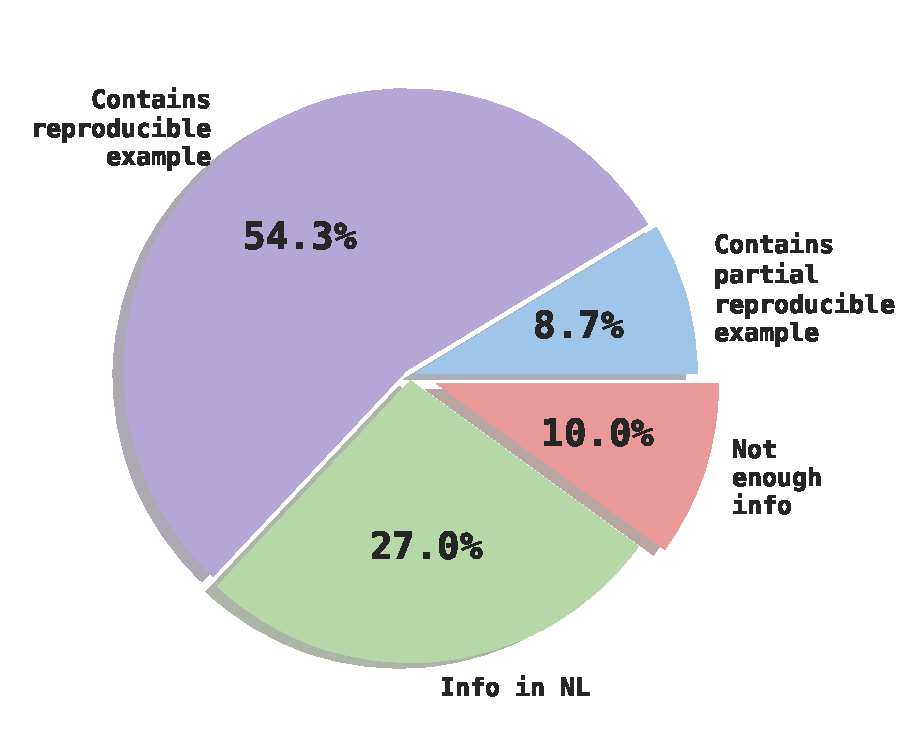
\includegraphics[width=\textwidth]{figs/benchmark_pie_description.pdf}
        \caption{Description quality}
        \label{fig:benchmark_description}
    \end{subfigure}
    \begin{subfigure}[b]{0.33\textwidth}
        \centering
        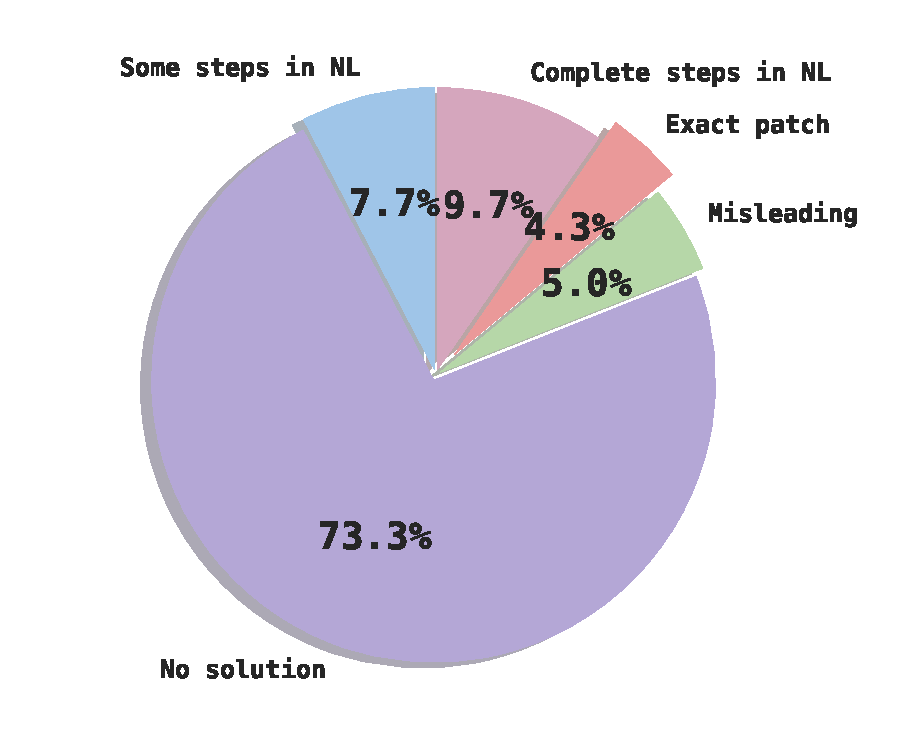
\includegraphics[width=\textwidth]{figs/benchmark_pie_patch.pdf}
        \caption{Solution in description}
        \label{fig:benchmark_patch}
    \end{subfigure}
    \begin{subfigure}[b]{0.32\textwidth}
        \centering
        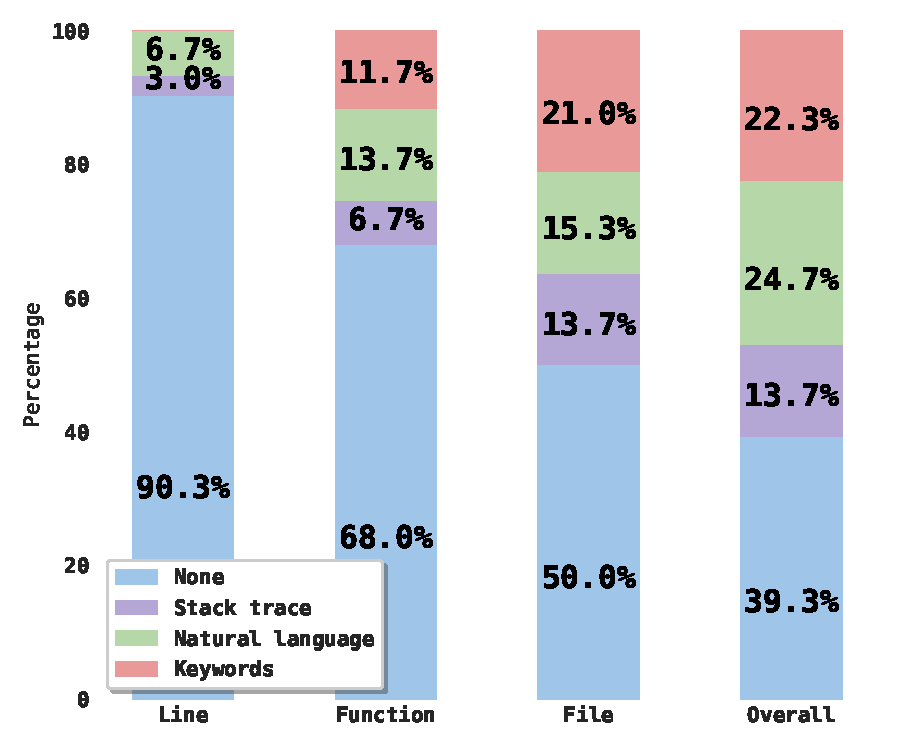
\includegraphics[width=\textwidth]{figs/benchmark_bar_location.pdf}
        \caption{Location information}
        \label{fig:benchmark_location}
    \end{subfigure}
    \caption{Categorization and corresponding breakdown of the \swebenchlite problems.} 
\end{figure*}

We now take a closer look at the problems in \swebenchlite. 
We first classify the existing problems to gain better understanding and additional insights on exactly what \emph{types} of problems \tech and prior approaches can solve. 
Specifically, we perform manual classification based on the issue description and ground truth developer patch of each problem.
Below describes each of classification dimensions and their categories in more detail:

\parabf{1) Description quality.} 
We first inspect whether each issue description contains sufficient information to perform the desired task. 
Figure~\ref{fig:benchmark_description} shows the distribution of each category: \emph{(i)} contains enough information in natural language, \emph{(ii)} contains reproducible failure example, \emph{(iii)} contains partially reproducible example, and \emph{(iv)} does not contain enough information.%
We observe that while a majority of the tasks in \swebenchlite contains  sufficient information, with many having some small failure examples to showcase the bug, there is a non-trivial percentage (\notenoughinfo) of problems which do not contain enough information.
Such problems include those that require implementing a new function with a specific name or adding an error message with a specific string that was not provided in the problem description.\footnote{These types of problems still exist in the benchmark despite claims that they have been completely removed by the filtering process according to \href{www.swebench.com/lite.html}{\swebenchlite}.}
This means the test will fail if the function name or error message string does not match exactly, even if the underlying functionality is correctly implemented.
Another example of insufficient information are problems that have multiple different interpretations on how to solve the issue, and only a subset of them can pass the ground truth test.
For instance, the issue description will outline two possible solutions suggestions with only one of them aligned well with developer intention.  
Implementing the other proposed solution suggestion will lead to test failure.
This highlights the necessity to further sanitize/improve \swebenchlite{} where these problems with uninformative descriptions shall be further excluded.



\parabf{2) Solution in description.} 
We also examine whether the solution or steps to solve the problem are already provided in the issue description.
Figure~\ref{fig:benchmark_patch} shows the breakdown of our categories: {\emph{(i)} no solution or steps provided, \emph{(ii)} partial solution provided (\eg some steps in natural language), \emph{(iii)} complete solution provided (\eg complete steps in natural language), \emph{(iv)} exact patch provided, and \emph{(v)} misleading solution or steps.} 
Interestingly, we observe that \exactpatch of issues contain the exact ground truth patch in the issue description, while an additional \stepsinnl of issues describe the exact steps required to come up with the correct solution. 
This shows that certain problems in \swebenchlite can be much easier to solve since they provide the solution either in exact code snippets or natural language. 
Furthermore, we also observe \misleadingpatch of issues contain proposed solution or steps in the issue description that do not reflect the ground truth patch introduced by the developers.
This further highlights potential issues with the benchmark, as these discrepancies can mislead tools to generate incorrect solutions simply by following the issue description. 


\parabf{3) Location information.} 
We further check if the issues description contains the correct location information. 
We divide the granularity into line, function, and file level. 
Our categories are: \emph{(i)} exact locations in natural language, \emph{(ii)} exact locations provided in failure stack traces, \emph{iii)} related keywords in the issue description that can be used to search for the location, and \emph{(iv)} not provided. 
We first observe that only in very few cases ($<$10\%), the issue provides the exact lines needed to fix the bug. 
However, this number increases as we increase the granularity to functions and files where we found that around half of the issues already provide the location of the file needed to be edited in the description.
To repair a bug or introduce a new feature, finding the location to make the edit is extremely important. 
As such, we leverage this classification and focus our later analysis on the effect the provided location has on the repair performance of \tech and baseline approaches.

These classification dimensions and categories raise potential issues with the \swebenchlite problems such as unsolvable questions, misleading potential solutions, and significant differences in problem difficulties.
These issues have not been properly considered by either the benchmark creation process or prior approaches. 
Furthermore, we hope our classification can provide additional insights on the type of problems that can be solved by existing and future approaches. 


\subsection{\swebenchlitefiltered}


\begin{table}[h]
\footnotesize
\centering
\caption{Performance and ranking on \swebenchlitefiltered. * indicates a tie in ranking.}
\label{tab:newbenchmark}
\scalebox{0.8}{
\begin{tabular}{ll|rlrl}
\toprule
     \multirow{2}*{Tool} & \multirow{2}*{\llm} & \multicolumn{2}{c}{\swebenchlite} & \multicolumn{2}{c}{\swebenchlitefiltered} \\
     & &  \%{} Resolved & Rank & \%{} Resolved & Rank \\
\midrule


\cellcolor[HTML]{e1ecff}\codestoryaide{}~\cite{codestoryaide} \lock{} & \cellcolor[HTML]{e1ecff}\makecell[l]{\openai{} \gptfouro{}+\anthropic{} \claudesonnet} & \cellcolor[HTML]{e1ecff}129 (43.00\%) & \cellcolor[HTML]{e1ecff}1 & \cellcolor[HTML]{e1ecff}114 (45.78\%) &\cellcolor[HTML]{e1ecff}1\\
\bytedanceagent{}~\cite{marscode} \lock{} & NA & 118 (39.33\%) & 2 & 106 (42.57\%) &2\\
\cellcolor[HTML]{e1ecff}\honeycomb{}~\cite{honeycomb} \lock{} & \cellcolor[HTML]{e1ecff}NA & \cellcolor[HTML]{e1ecff}115 (38.33\%) & \cellcolor[HTML]{e1ecff}3 & \cellcolor[HTML]{e1ecff}98 (39.36\%) &\cellcolor[HTML]{e1ecff}3\\
\mentatbot{}~\cite{mentatbot} \lock{} & \openai{} \gptfouro{} & 114 (38.00\%) & 4 & 96 (38.55\%) &4\\
\cellcolor[HTML]{e1ecff}\gru{}~\cite{gru} \lock{} & \cellcolor[HTML]{e1ecff}NA & \cellcolor[HTML]{e1ecff}107 (35.67\%) & \cellcolor[HTML]{e1ecff}5 & \cellcolor[HTML]{e1ecff}94 (37.75\%) &\cellcolor[HTML]{e1ecff}5\\
\isoform{}~\cite{isoform} \lock{} & NA & 105 (35.00\%) & 6 & 91 (36.55\%) &6\\
\cellcolor[HTML]{e1ecff}\supercoder{}~\cite{supercoder} \lock{} & \cellcolor[HTML]{e1ecff}NA & \cellcolor[HTML]{e1ecff}102 (34.00\%) & \cellcolor[HTML]{e1ecff}7 & \cellcolor[HTML]{e1ecff}87 (34.94\%) &\cellcolor[HTML]{e1ecff}7\\
\lingma{}~\cite{lingma} \lock{} & \makecell[l]{\openai{} \gptfouro{}+\anthropic{} \claudesonnet} & 99 (33.00\%) & 8 & 86 (34.54\%) &8\\
\cellcolor[HTML]{e1ecff}\factorydroid{}~\cite{factorydroid} \lock{} & \cellcolor[HTML]{e1ecff}NA & \cellcolor[HTML]{e1ecff}94 (31.33\%) & \cellcolor[HTML]{e1ecff}10 & \cellcolor[HTML]{e1ecff}82 (32.93\%) &\cellcolor[HTML]{e1ecff}10\\
\amazonqagent{}-v2~\cite{amazonqdeveloper} \lock{} & NA & 89 (29.67\%) & 12* & 76 (30.52\%) &13\\
\cellcolor[HTML]{e1ecff}\coder{}~\cite{coder} \lock{} & \cellcolor[HTML]{e1ecff}\openai{} \gptfour{} & \cellcolor[HTML]{e1ecff}85 (28.33\%) & \cellcolor[HTML]{e1ecff}14 & \cellcolor[HTML]{e1ecff}71 (28.51\%) &\cellcolor[HTML]{e1ecff}14*\\
\masai{}~\cite{masai} \lock{} & NA & 84 (28.00\%) & 15 & 70 (28.11\%) &16\\
\cellcolor[HTML]{e1ecff}\sima{}~\cite{sima} \lock{} & \cellcolor[HTML]{e1ecff}\openai{} \gptfouro{} & \cellcolor[HTML]{e1ecff}83 (27.67\%) & \cellcolor[HTML]{e1ecff}16 & \cellcolor[HTML]{e1ecff}71 (28.51\%) &\cellcolor[HTML]{e1ecff}14*\\
\ibmagent{}~\cite{ibmagent} \lock{} & NA & 80 (26.67\%) & 17* & 66 (26.51\%) &18*\\
\cellcolor[HTML]{e1ecff}\opencsgagent{}~\cite{opencsgstarship} \lock{} & \cellcolor[HTML]{e1ecff}\openai{} \gptfour{} & \cellcolor[HTML]{e1ecff}71 (23.67\%) & \cellcolor[HTML]{e1ecff}22 & \cellcolor[HTML]{e1ecff}56 (22.49\%) &\cellcolor[HTML]{e1ecff}23*\\
\amazonqagent{}~\cite{amazonqdeveloper} \lock{} & NA & 61 (20.33\%) & 26 & 51 (20.48\%) &25*\\
\cellcolor[HTML]{e1ecff}\repounderstander{}~\cite{repounderstander} \lock{} & \cellcolor[HTML]{e1ecff}\openai{} \gptfour{} & \cellcolor[HTML]{e1ecff}64 (21.33\%) & \cellcolor[HTML]{e1ecff}25 & \cellcolor[HTML]{e1ecff}51 (20.48\%) &\cellcolor[HTML]{e1ecff}25*\\
\midrule
\autocoderover{}-v2~\cite{autocoderovertwo} & \openai{} \gptfouro{} & 92 (30.67\%) & 11 & 79 (31.73\%) &11\\
\cellcolor[HTML]{e1ecff}\repograph~\cite{repograph} & \cellcolor[HTML]{e1ecff}\openai{} \gptfouro{} & \cellcolor[HTML]{e1ecff}89 (29.67\%) & \cellcolor[HTML]{e1ecff}12* & \cellcolor[HTML]{e1ecff}77 (30.92\%) &\cellcolor[HTML]{e1ecff}12\\
\multirow{1}*{\moatless{}~\cite{moatless}} & \anthropic{} \claudesonnet{} & 80 (26.67\%) & 17* & 67 (26.91\%) &17\\
 & \openai{} \gptfouro{} & 74 (24.67\%) & 21 & 62 (24.90\%) &21\\
\cellcolor[HTML]{e1ecff}\opendevincodeact{}~\cite{opendevin} & \cellcolor[HTML]{e1ecff}\anthropic{} \claudesonnet & \cellcolor[HTML]{e1ecff}80 (26.67\%) & \cellcolor[HTML]{e1ecff}17* & \cellcolor[HTML]{e1ecff}65 (26.10\%) &\cellcolor[HTML]{e1ecff}20\\
\aider{}~\cite{aidar} & \makecell[l]{\openai{} \gptfouro{}+\anthropic{} \claudesonnet} & 79 (26.33\%) & 20 & 66 (26.51\%) &18*\\
\cellcolor[HTML]{e1ecff}\multirow{1}*{\sweagent{}~\cite{sweagent}} & \cellcolor[HTML]{e1ecff}\anthropic{} \claudesonnet{} & \cellcolor[HTML]{e1ecff}69 (23.00\%) & \cellcolor[HTML]{e1ecff}23 & \cellcolor[HTML]{e1ecff}58 (23.29\%) &\cellcolor[HTML]{e1ecff}22\\
\cellcolor[HTML]{e1ecff} & \cellcolor[HTML]{e1ecff}\openai{} \gptfouro{} & \cellcolor[HTML]{e1ecff}55 (18.33\%) & \cellcolor[HTML]{e1ecff}28 & \cellcolor[HTML]{e1ecff}45 (18.07\%) &\cellcolor[HTML]{e1ecff}27*\\
\cellcolor[HTML]{e1ecff} & \cellcolor[HTML]{e1ecff}\openai{} \gptfour{} & \cellcolor[HTML]{e1ecff}54 (18.00\%) & \cellcolor[HTML]{e1ecff}29 & \cellcolor[HTML]{e1ecff}42 (16.87\%) &\cellcolor[HTML]{e1ecff}29\\
\appmapnavie{}~\cite{appmapnavie} & \openai{} \gptfouro{} & 65 (21.67\%) & 24 & 56 (22.49\%) &23*\\
\cellcolor[HTML]{e1ecff}\autocoderover{}~\cite{autocoderover} & \cellcolor[HTML]{e1ecff}\openai{} \gptfour{} & \cellcolor[HTML]{e1ecff}57 (19.00\%) & \cellcolor[HTML]{e1ecff}27 & \cellcolor[HTML]{e1ecff}45 (18.07\%) &\cellcolor[HTML]{e1ecff}27*\\
\midrule
\rag{}~\cite{sweagent} & \anthropic{} \claudeopus{} & 13 (4.33\%) & 30 & 10 (4.02\%) &30\\
 & \openai{} \gptfour{} & 8 (2.67\%) & 32 & 5 (2.01\%) &32\\
 & \anthropic{} \claude{}-2 & 9 (3.00\%) & 31 & 6 (2.41\%) &31\\
 & \openai{} \chatgpt{} & 1 (0.33\%) & 33 & 0 (0.00\%) &33\\
 \midrule
\cellcolor[HTML]{e1ecff}\textbf{\tech{}} & \cellcolor[HTML]{e1ecff}\openai{} \gptfouro{} & \cellcolor[HTML]{e1ecff}96 (32.00\%) & \cellcolor[HTML]{e1ecff}9 & \cellcolor[HTML]{e1ecff}84 (33.73\%) &\cellcolor[HTML]{e1ecff}9\\


\bottomrule
\end{tabular}
}
\end{table}

Building on the above problem classifications, we will more rigorously compare and contrast \tech and existing work. 
Specifically, we focus on a subset of the problems in \swebenchlite after removing the problems that contain the exact patch in the problem description, misleading solutions, or do not provide enough information in the original issue description.  
This eliminates the less reasonable problems and normalizes the difficulty level of the benchmark. 
We refer to our subset of \sanitizedtotalproblem{} problems as \swebenchlitefiltered{}. 
We note here that our approach of identifying and excluding problematic problems has already been confirmed by a later work done by OpenAI, where they have released a similar filtered benchmark of \swebenchverified~\cite{openaiverified}.  





Table~\ref{tab:newbenchmark} shows the results on the \swebenchlitefiltered{} benchmark and the corresponding ranking of each approach.
We also included the results on the original 300 problems in \swebenchlite for comparison. 
While the general ranking of all approaches stay roughly the same, we do observe some small ranking changes.
%
Compared to the original \swebenchlite, our filtered benchmark of \swebenchlitefiltered provides a more accurate reflection of the true capability of autonomous software development tools. 


\begin{figure*}[h]
\centering
    \begin{subfigure}[b]{0.32\textwidth}
        \centering
        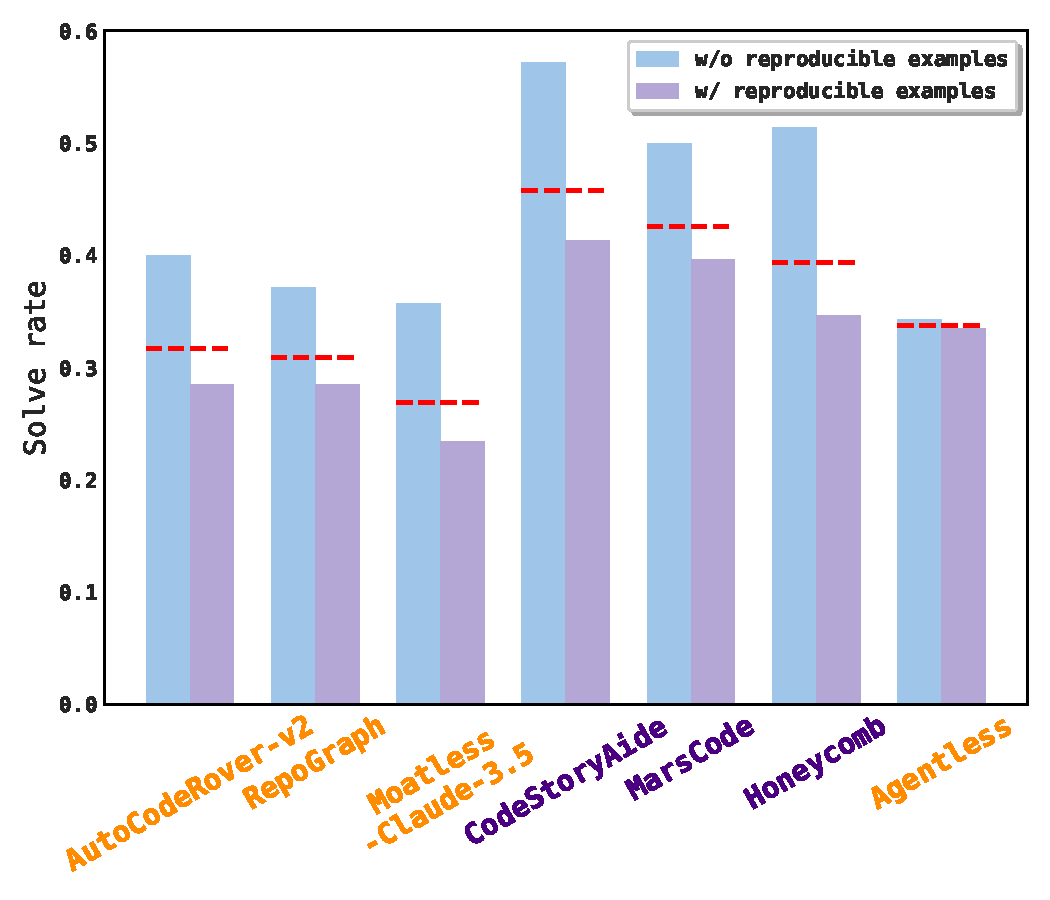
\includegraphics[width=\textwidth]{figs/filtered_benchmark_comparison.pdf}
        \caption{Description quality}
        \label{fig:filered_benchmark_description}
    \end{subfigure}
    \begin{subfigure}[b]{0.32\textwidth}
        \centering
        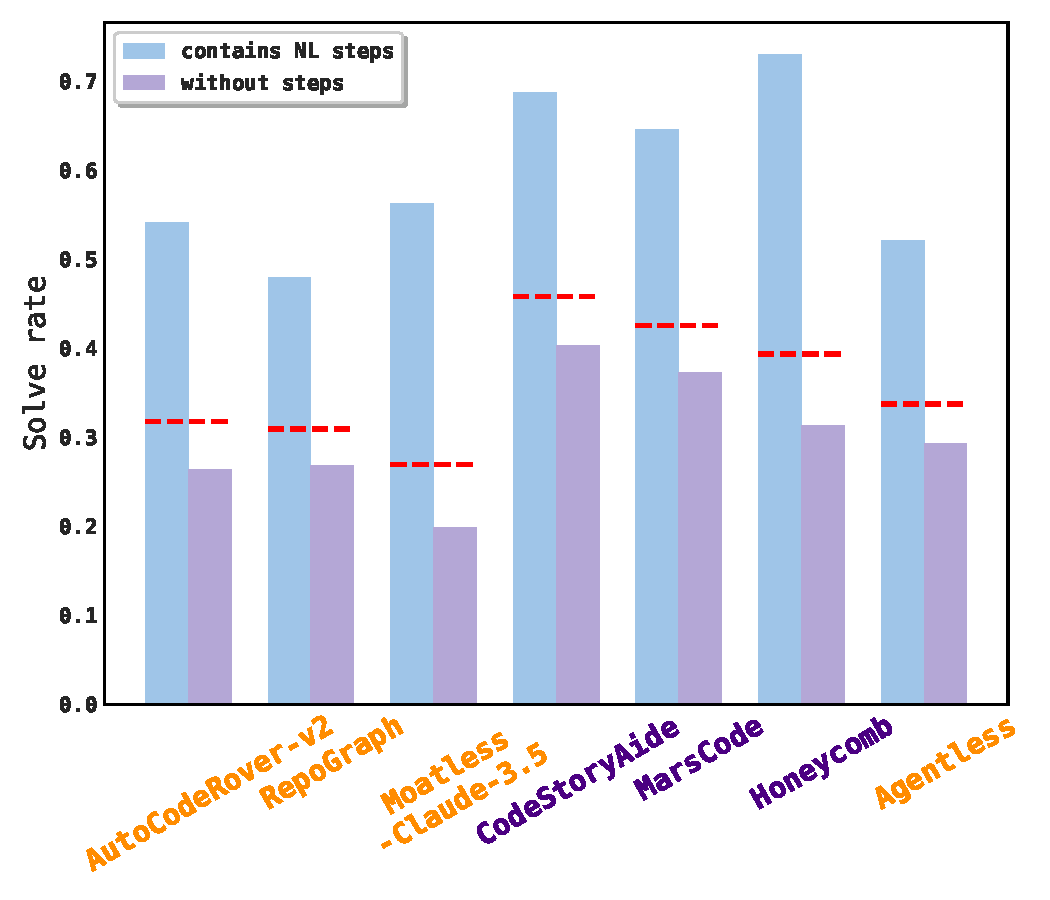
\includegraphics[width=\textwidth]{figs/filtered_benchmark_patch_comparison.pdf}
        \caption{Solution in description}
        \label{fig:filered_benchmark_patch}
    \end{subfigure}
    \begin{subfigure}[b]{0.32\textwidth}
        \centering
        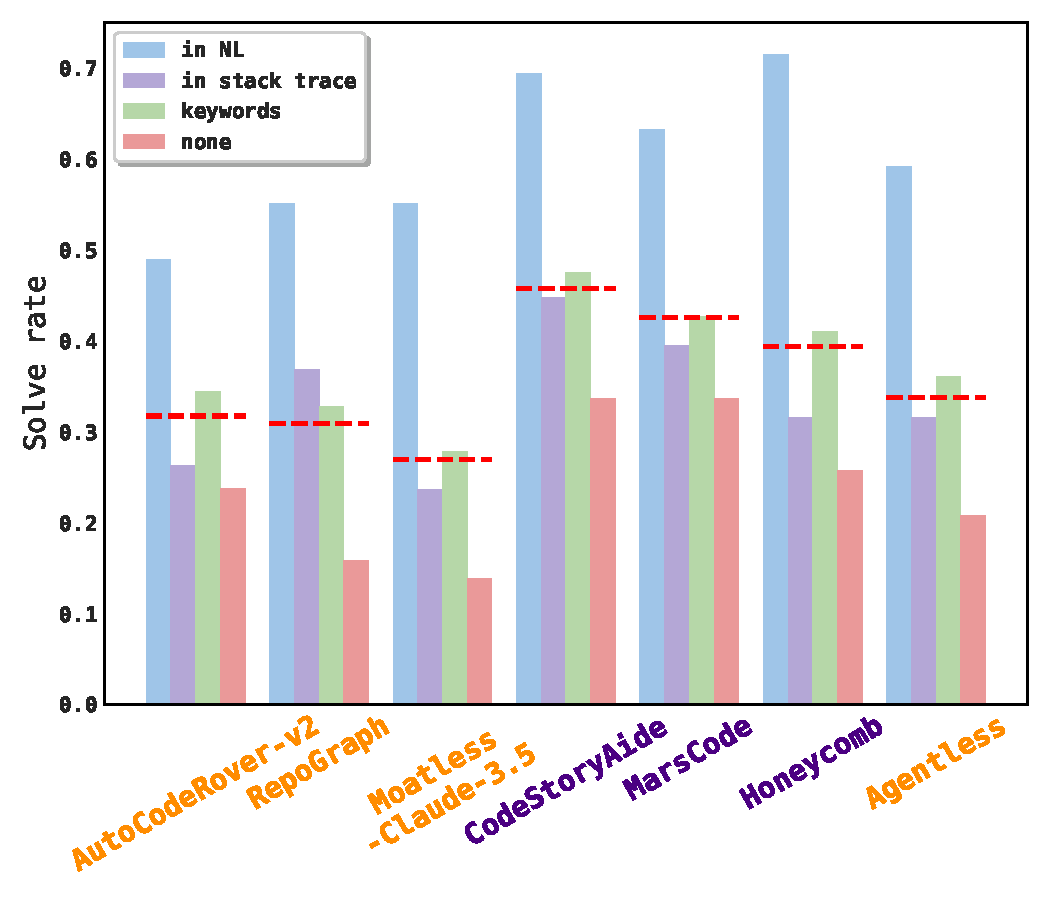
\includegraphics[width=\textwidth]{figs/filtered_benchmark_location_comparison.pdf}
        \caption{Location information}
        \label{fig:filtered_benchmark_location}
    \end{subfigure}
    \caption{Solve rate of selected approaches (\textbf{\textcolor[HTML]{db8500}{orange}} means open-source while \textbf{\textcolor[HTML]{2e0063}{indigo}} means closed-source) on different problem categories in \swebenchlitefiltered{}. \textcolor{red}{Red} dotted line indicates the average solve rate on the entire \swebenchlitefiltered for each approach.
    } 
    \label{fig:filtered_comparison}
\end{figure*}




Using the classification results, we further examine the types of problems that are solved by \tech and prior approaches on \swebenchlitefiltered. 
Figure~\ref{fig:filtered_comparison} shows the solve rate of various top-performing open-source and closed-source approaches across the different categories of problems. 
We first examine if having code examples to reproduce the error in the issue description can help the \llm better solve the issue in Figure~\ref{fig:filered_benchmark_description}.
Surprisingly, we found that the solve rate of all prior approaches drop when evaluated on the problems with reproducible code examples.
Many agent-based approaches~\cite{sweagent, opendevin, coder} attempt to first reproduce the error, however, this may not improve performance even on problems with already provided reproducible examples. 
However, we observe the performance for \tech remains very high on the problems with reproducible code examples. 
This is because \tech generates \reproduction tests using the original issues descriptions, hence can better make use of the reproducible code examples provided (similarly for \mentatbot{} which also contains an explicit test generation step).
This demonstrate the importance of the test generation stage for patch selection.
Next, we look at the effect of ground truth patch/solution in the issue description. 
Figure~\ref{fig:filered_benchmark_patch} shows the expected result where all selected techniques perform better on issues that already provide solution steps in natural language. 
Furthermore, in Figure~\ref{fig:filtered_benchmark_location}, we examine the solve rate with respect to the location information provided in the issues description.
Unsurprisingly, we found that the highest solve rates are on problems where the location is provided in natural language followed by stack traces. 
The most difficult problems are those that do not contain any clues about the location of the issue in the description.
We observe that compared with closed-source approaches, \tech performs comparably when the location is provided in either natural language, stack trace, or keywords. 
However, the closed-source agent tools perform better compared to \tech in the case where no location clue is provided.
This highlights an advantage of agent-based tools in solving these more complex problems where they are able to use complex code search tools. 
This represents potential future work for \tech to target and further improve these types of problems. 


















\subsection{\swebenchverified}

\begin{table}[h]
\footnotesize
\centering
\caption{Performance on \swebenchverified.}
\label{tab:swebenchverified}
\scalebox{0.9}{
\begin{tabular}{ll|r}
\toprule
 Tool & \llm & \%{} Resolved \\
\midrule

\cellcolor[HTML]{e1dcef}\multirow{1}*{\toolstool{}~\cite{tools} \lock{}} & \cellcolor[HTML]{e1dcef}\anthropic{} \claudesonnet{}onnet (20241022) & \cellcolor[HTML]{e1dcef}245 (49.00\%) \\
\cellcolor[HTML]{e1dcef} & \cellcolor[HTML]{e1dcef}\anthropic{} \claudehaiku{} & \cellcolor[HTML]{e1dcef}203 (40.60\%) \\
\solversolver{}~\cite{solver} \lock{} & NA & 227 (45.40\%) \\
\cellcolor[HTML]{e1dcef}\gru{}~\cite{gru} \lock{} & \cellcolor[HTML]{e1dcef}NA & \cellcolor[HTML]{e1dcef}226 (45.20\%) \\
\honeycomb{}~\cite{honeycomb} \lock{} & NA & 203 (40.60\%) \\
\cellcolor[HTML]{e1dcef}\amazonqagent{}-v2~\cite{amazonqdeveloper} \lock{} & \cellcolor[HTML]{e1dcef}NA & \cellcolor[HTML]{e1dcef}194 (38.80\%) \\
\factorydroid{}~\cite{factorydroid} \lock{} & NA & 185 (37.00\%) \\
\cellcolor[HTML]{e1dcef}\amazonqagent{}~\cite{amazonqdeveloper} \lock{} & \cellcolor[HTML]{e1dcef}NA & \cellcolor[HTML]{e1dcef}128 (25.60\%) \\
\midrule
\composio{}~\cite{composio} & \anthropic{} \claudesonnet{}onnet & 203 (40.60\%) \\
\cellcolor[HTML]{e1dcef}\autocoderover{}-v2~\cite{autocoderovertwo} & \cellcolor[HTML]{e1dcef}\openai{} \gptfouro{} & \cellcolor[HTML]{e1dcef}192 (38.40\%) \\
\multirow{1}*{\sweagent{}~\cite{sweagent}} & \anthropic{} \claudesonnet{}onnet & 168 (33.60\%) \\
 & \openai{} \gptfouro{} & 116 (23.20\%) \\
 & \openai{} \gptfour{} & 112 (22.40\%) \\
\cellcolor[HTML]{e1dcef}\lingma{}~\cite{lingma} & \cellcolor[HTML]{e1dcef}\lingmaswegpt & \cellcolor[HTML]{e1dcef}144 (28.80\%) \\
\appmapnavie{}~\cite{appmapnavie} & \openai{} \gptfouro{} & 131 (26.20\%) \\
\midrule
\textbf{\tech} & \openai{} \gptfouro{} & 194 (38.80\%) \\ 
\bottomrule
\end{tabular}
}
\end{table}

Similar to \swebenchlitefiltered{} and inspired by similar concerns in Section~\ref{sec:benchmark_analysis}, OpenAI has produced a newly filtered dataset of \swebenchverified~\cite{openaiverified} validated by human developers to ensure each issue has sufficient amounts of information to be solved. 
Table~\ref{tab:swebenchverified} shows the performance of \tech compared with prior agent-based approaches on \swebenchverified. 
Similar to the results on \swebenchlite, \tech maintains its strong performance and is able to solve 194 out of 500 problems (38.80\%). 
\tech is able to achieve the second highest performance compared with open-source approaches and perform better than many closed-source / commercial techniques. 
Furthermore, we note that \tech performs the best among all techniques that use \gptfouro as the \llm. 
